%!TEX ROOT=formularioFisica.tex

\section{Onde}\label{sec:onde}
Questa sezione si dedica alle formule ed esperimenti relativi allo studio del moto ondoso dei 
corpi. Luci e suoni sono esempi di onde e oscillazioni, uno dei fenomeni più diffusi in
natura. Le onde si propagano nello spazio e permettono di trasportare anche enormi quantità di
energia, ma non massa.

\begin{center}
  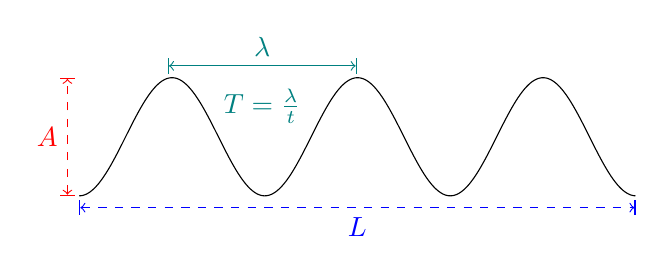
\begin{tikzpicture}[scale=0.75]
    \draw[samples=500, domain=-0:pi*3] plot (\x, {-cos(2*\x r)});

    \draw[|<->|, blue, dashed] (0,-1.2) -- (9.42,-1.2)
      node[pos=0.5, below]{$L$};
    \draw[|<->|, red, dashed] (-0.2, -1) -- (-0.2, 1)
      node[pos=0.5, left]{$A$};
    \draw[|<->|, teal] (1.5, 1.2) -- (4.7, 1.2)
      node[pos=0.5, above]{$\lambda$}
      node[pos=0.5, anchor=north, yshift=-5]{$T = \frac{\lambda}{t}$};
  \end{tikzpicture}
\end{center}
Il grafico qua sopra è il grafico della funzione $\cos x$ che rappresenta un possibile moto di un'
onda. Sono anche rappresentate le 3 caratteristiche principali: l'\emph{ampiezza}
($\mathcolor{red}{A}$), la \emph{lunghezza} ($\mathcolor{blue}{L}$) e la \emph{lunghezza d'onda}
($\mathcolor{teal}{\lambda}$).\\[\baselineskip]
Per gli esercizi, si vada a pagina~\pageref{ex:onde}.

\subsection{Velocità di propagazione} \label{subsec:onde:sper}
Di seguito vengono riportate formule sperimentali da usare ad esempio con una corda che oscilla.
\begin{equation*}
  v = \sqrt{\frac{T}{\mu}}
\end{equation*}
\begin{equation*}
  \mu = \frac{m}{\mathcolor{blue}{L}}
\end{equation*}
$T$: tensione della corda\\
$\mu$: densità lineare della corda\\
$m$: massa della corda\\
$\mathcolor{blue}{L}$: lunghezza della corda

\subsection{Relazione fondamentale}
\begin{equation*}
  v = \frac{\mathcolor{teal}{\lambda}}{T} = \mathcolor{teal}{\lambda}f
\end{equation*}
Questa formula mette in relazione la velocità, il periodo, la lunghezza d'onda e la frequenza
di oscillazione.

\subsection{Equazioni dell'onda}
Esistono più equazioni dell'onda, dalla più generale alle due particolari.

\subsubsection{Equazione con $x$ fissato}
Questa formula definisce l'equazione dell'onda in un punto fisso.
\begin{equation*}
  f(\bar{x}, t) = \mathcolor{red}{A}\cos\frac{2\pi}{T}t
\end{equation*}

\subsubsection{Equazione con $t$ fissato}
Questa formula definisce l'equazione dell'onda ad un particolare istante.
\begin{equation*}
  f(x, \bar{t}) = \mathcolor{red}{A} \cos\frac{2\pi}{\mathcolor{teal}{\lambda}}x
\end{equation*}

\subsubsection{Equazione generale del'onda}
Queste sono le formule più generali dell'equazione dell'onda.
\begin{equation*}
  f(x, t) = \mathcolor{red}{A}\cos\left[\frac{2\pi}{\mathcolor{teal}{\lambda}}(x\mp vt)\right] =
  \mathcolor{red}{A}\cos2\pi\left(\frac{x}{\mathcolor{teal}{\lambda}}\mp\frac{t}{T}\right)
\end{equation*}

La cosa più importante da notare è il segno. Se l'onda si propaga a \emph{destra} si usi $-$, se
verso \emph{sinistra} si usi $+$.

\subsection{Equazione di Huygens}
L'equazione di Huygens definisce il rapporto tra il raggio di propagazione di un onda e il tempo.
La seguente figura farà capire meglio.

\begin{center}
  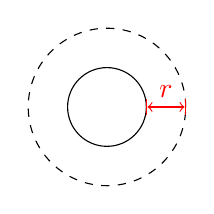
\begin{tikzpicture}[scale=0.5]
    \draw (0,0) circle (1);
    \draw[dashed] (0,0) circle (2);

    \draw[|<->|, red] (1,0) -- (2,0)
      node[pos=0.5, above]{$r$};
  \end{tikzpicture}
\end{center}
\begin{equation*}
  \mathcolor{red}{r} = \Delta t\cdot v
\end{equation*}
$v$: velocità di propagazione

\subsection{Luce}
La luce è un'onda (precisamente è un'onda elettromagnetica). La luce trasporta energia e per 
determinare l'intensità di una luce ad una certa distanza si definisce l'irradiamento
\begin{equation*}
  I = \frac{E}{\Delta tS} = \frac{P}{S}
\end{equation*}
$E$: energia della sorgente\\
$S$: superficie investita dalla luce ($4\pi r^2$)\\
$P$: potenza


\subsection{Polarizzazione}
Polarizzare un'onda significa ``selezionare'' una parte e bloccarne un'altra.
\subsubsection{Legge di Malus}
I polaroid sono dei filtri polarizzatori, caratterizzati da un'asse di trasmissione.\\
La legge di Malus definisce l'intensità dell'onda dopo il polaroid a seconda se la sorgente
è polarizzata o meno.
\begin{center}
  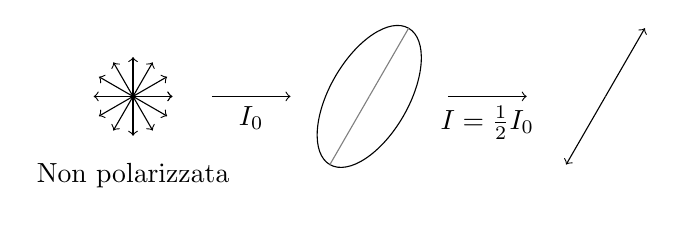
\begin{tikzpicture}
    \foreach \a in {0,30,60,...,360}{
      \draw[->] (0,0) -- (\a:0.5);
    }
    \draw[->] (1,0) -- (2,0)
      node[pos=0.5,below]{$I_0$};
    \filldraw[draw=black,fill=white,rotate around={-30:(3,0)}] (3,0) ellipse (0.5 and 1);
    \draw[thin,gray] (3,0) -- ++(60:1);
    \draw[thin,gray] (3,0) -- ++(240:1);
    \draw[->] (4,0) -- (5,0)
      node[pos=0.5,below]{$I = \frac{1}{2}I_0$};
    \node at (0,-1) {Non polarizzata};
    \draw [->] (6,0) -- ++(60:1);
    \draw [->] (6,0) -- ++(240:1);
  \end{tikzpicture}
\end{center}
Queta vale se la sorgente di luce non è polarizzata, quindi una lampadina ad esempio.
\begin{center}
  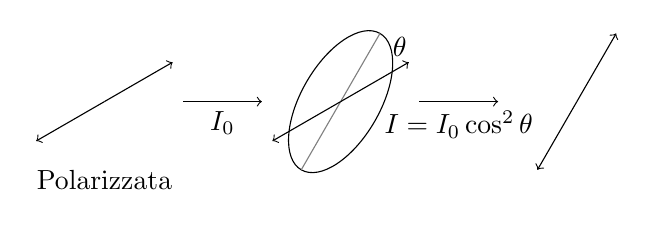
\begin{tikzpicture}
    \draw[->](0,0) -- ++(30:1);
    \draw[->] (0,0) -- ++(210:1);
    \draw[->] (1,0) -- (2,0)
      node[pos=0.5,below]{$I_0$};
    \filldraw[draw=black,fill=white,rotate around={-30:(3,0)}] (3,0) ellipse (0.5 and 1);
    \draw[thin,gray](3,0) -- coordinate(A) ++(60:1);
    \draw[thin,gray] (3,0) -- ++(240:1);
    \draw[->](3,0) -- coordinate (B) ++(30:1);
    \draw[->] (3,0) -- ++(210:1);
    \coordinate (A) at (3.5,0.86);
    \coordinate (O) at (3,0);
    \coordinate (B) at (3.86,0.5);
    \markangle{O}{A}{B}{0.6}{1.2}{$\text{ }$}
    \node at (3.75,0.7) {$\theta$};
    \draw[->] (4,0) -- (5,0)
      node[pos=0.5,below]{$I = I_0\cos^2\theta$};
    \node at (0,-1) {Polarizzata};
    \draw[->] (6,0) -- ++(60:1);
    \draw[->] (6,0) -- ++(240:1);
  \end{tikzpicture}
\end{center}
$\theta$: angolo tra l'asse di trasmissione e quello della luce polarizzata

\subsubsection{Angolo di Brewster}
Ogni raggio riflesso e rifratto è parzialmente polarizzato. L'angolo di Brewster è quel particolare
angolo in cui la polarizzazione è massima ed è rappresentato dal seguente disegno.
\begin{center}
  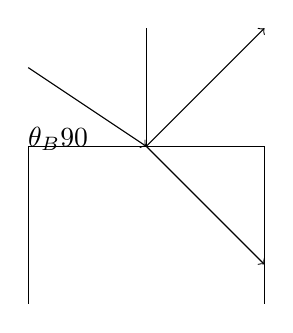
\begin{tikzpicture}
    \draw (0,-2) -- (0,0) -- ++(3,0) -- ++(0,-2);
    \coordinate (In) at (0,1);
    \coordinate (Center) at (1.5,0);
    \coordinate (OutB) at (3,1.5);
    \coordinate (OutR) at (3,-1.5);
    \coordinate (OutM) at (1.5,1.5);
    \draw[->] (In) -- (Center);
    \draw[->] (Center) -- (OutB);
    \draw[->] (Center) -- (OutR);
    \draw (Center) -- (OutM);
    \markangle[cyan]{Center}{In}{OutM}{1}{1.5}{$\theta_B$}
    \markangle[orange]{Center}{OutB}{OutR}{1}{1.5}{$\ang{90}$}
  \end{tikzpicture}
\end{center}
Dato che gli indici di rifrazione sono diversi, possiamo scrivere per la relazione di Snell
\begin{equation*}
  n_1\sin\theta_B = n_2\sin\hat{r}
\end{equation*}
e vedendo che $\hat{r} = 90-\theta_B$ e quindi
\begin{equation*}
  n_1\sin\theta_B = n_2\sin(90-\theta_B) = \cos\theta_B
\end{equation*}
E quindi
\begin{equation*}
  \theta_B = \arctan\frac{n_2}{n_1}
\end{equation*}

\subsection{Rifrazione}\label{subsec:onde:rifrazione}
Questa sezione si occuperà della luce rifratta/riflessa.\\
Per gli esercizi si vada a pagina~\pageref{ex:rifrazione}.\\ [\baselineskip]
In questa sezione è fondamentale l'\emph{indice di rifrazione}.\\
Per calcolarlo si usi:
\begin{equation*}
  n_{2,1} = \frac{\sin\hat{i}}{\sin\hat{r}} = \frac{n_2}{n_1}
\end{equation*}
Qui introduciamo anche due simboli: $\hat{i}$ e $\hat{r}$. Il primo ($\hat{i}$) indica l'angolo di
\emph{incidenza} con il secondo mezzo e $\hat{r}$ l'angolo di rifrazione. Per capire meglio, si
faccia riferimento alla seguente figura:

\begin{center}
  \begin{tikzpicture}[scale=0.6]
    \coordinate (A) at (-2,1);
    \coordinate (B) at (2,1);
    \coordinate (C) at (2,-1);
    \coordinate (D) at (-2,-1);

    \coordinate (In) at (-1,-1);
    \coordinate (Out) at (1, 1);

    % Rectangle
    \draw (A) -- (B) -- (C) -- (D) -- cycle;
    % Angles
    \filldraw[orange, fill=orange!30] (In) -- ($(In) + (0, -0.6)$) arc(-90:-105:1) -- cycle;
    \draw[orange] (In) +(-97:1) node{$\hat{i}$};
    \filldraw[cyan, fill=cyan!30] (In) -- ($(In) + (0, 0.6)$) arc(90:61:1) -- cycle;
    \draw[cyan] (In) +(80:1) node{$\hat{r}$};
    % Construction lines
    \draw[densely dotted] ($(In) + (0, -0.5)$) -- ++(0,2.5);
    \draw[densely dotted]($(Out) + (0, 0.5)$) -- ++(0,-2.5);
    \draw[dashed, -latex] (In) -- (Out);
    % In line
    \draw[-latex] (-1.5,-2) -- (In);
    \draw[-latex] (Out) -- (1.5, 2);
    %\draw[|<->|, blue] ($(In) + (0, 2.2)$) -- ($(Out) + (0, 0.2)$)
    %	node[pos=0.5, above]{$\delta$};
    %\draw[|<->|, red] ($(A) + (-0.2,0)$) -- ($(D) + (-0.2,0)$)
    %	node[pos=0.5, left]{$d$};
  \end{tikzpicture}
\end{center}

Si tenga conto che questa immagine si riferisce al fenomeno della \emph{rifrazione} che ha queste
caratteristiche:
\begin{equation*}
  \frac{\sin\mathcolor{orange}{\hat{i}}}{\sin\mathcolor{cyan}{\hat{r}}} = \frac{v_1}{v_2} = 
  \frac{\lambda_1}{\lambda_2} = \frac{c}{v_2}
\end{equation*}
Da notare che $\dfrac{c}{v_2}$ vale solo se la luce dal vuoto passa in un altro mezzo.\\
%\subsubsection{Relazione di Snell}
%La relazione di Snell mette appunto in relazione gli indici di rifrazione con gli angoli $\hat{i}$ 
%e $\hat{r}$.
%\begin{equation*}
%  \frac{n_2}{n_1} = \frac{\sin\mathcolor{orange}{\hat{i}}}{\sin\mathcolor{cyan}{\hat{r}}}
%\end{equation*}

\subsubsection{Riflessione}
\begin{equation*}
  \mathcolor{orange}{\hat{i}} =\mathcolor{cyan}{\hat{r}}
\end{equation*}
\begin{center}
  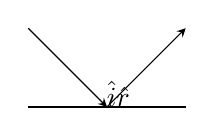
\begin{tikzpicture}
    \coordinate (O) at (0,0);
    \coordinate (A) at (-1,1);
    \coordinate (B) at (1,1);
    \coordinate (M1) at (-1,0);
    \coordinate (M2) at (1,0);

    \draw (-1,0) -- ++(2,0);
    \draw[-stealth] (A) -- (O);
    \draw[-stealth] (O) -- (B);
    \markangle[orange]{O}{A}{M1}{0.5}{1.5}{$\hat{i}$}
    \markangle[cyan]{O}{B}{M2}{0.5}{1.5}{$\hat{r}$}
  \end{tikzpicture}
\end{center}

\subsubsection{Scostamento del raggio}
\begin{center}
  \begin{tikzpicture}[scale=0.6]
    \coordinate (A) at (-2,1);
    \coordinate (B) at (2,1);
    \coordinate (C) at (2,-1);
    \coordinate (D) at (-2,-1);

    \coordinate (In) at (-1,-1);
    \coordinate (Out) at (1, 1);

    % Rectangle
    \draw (A) -- (B) -- (C) -- (D) -- cycle;
    % Angles
    \filldraw[orange, fill=orange!30] (In) -- ($(In) + (0, -0.6)$) arc(-90:-105:1) -- cycle;
    \draw[orange] (In) +(-97:1) node{$\hat{i}$};
    \filldraw[cyan, fill=cyan!30] (In) -- ($(In) + (0, 0.6)$) arc(90:61:1) -- cycle;
    \draw[cyan] (In) +(80:1) node{$\hat{r}$};
    % Construction lines
    \draw[densely dotted] ($(In) + (0, -0.5)$) -- ++(0,2.5);
    \draw[densely dotted]($(Out) + (0, 0.5)$) -- ++(0,-2.5);
    \draw[dashed, -latex] (In) -- (Out);
    % In line
    \draw[-latex] (-1.5,-2) -- (In);
    \draw[-latex] (Out) -- (1.5, 2);
    \draw[dashed] (In) -- (0,1);
    \draw[|<->|, olive] (0,1) -- (0.6,0.65)
      node[pos=0.5, below left]{$\gamma$};

    \draw[|<->|, blue] ($(In) + (0, 2.2)$) -- ($(Out) + (0, 0.2)$)
      node[pos=0.5, above]{$\delta$};
    \draw[|<->|, red] ($(A) + (-0.2,0)$) -- ($(D) + (-0.2,0)$)
      node[pos=0.5, left]{$d$};
  \end{tikzpicture}
\end{center}

\begin{equation*}
  \mathcolor{blue}{\delta} = \frac{\mathcolor{red}{d}\sin(
  \mathcolor{orange}{\hat{i}}-\mathcolor{cyan}{\hat{r}})}
  {\cos\mathcolor{cyan}{\hat{r}}}
\end{equation*}
\begin{equation*}
  \mathcolor{olive}{\gamma} = \mathcolor{red}{d}\tan\mathcolor{cyan}{\hat{r}}
\end{equation*}

\subsubsection{Angolo limite}
L'angolo limite è quell'angolo che segna il passaggio da un fenomeno di rifrazione a uno di 
riflessione o viceversa.
\begin{equation*}
  \hat{a}_l = \arcsin\frac{n_2}{n_1}
\end{equation*}

\subsubsection{Immagine riassuntiva}
\begin{center}
  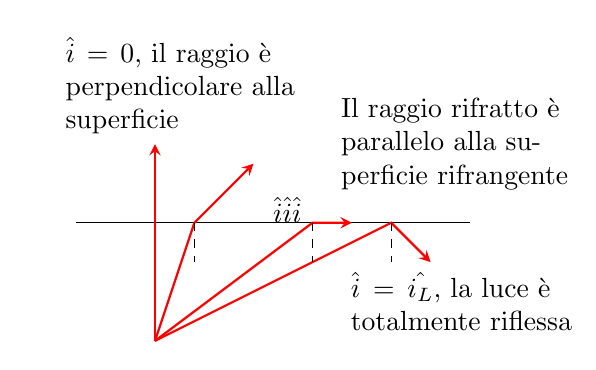
\begin{tikzpicture}[scale=0.5]
    \coordinate (L) at (-5,0);
    \coordinate (R) at (5,0);
    \coordinate (A) at (-3,0);
    \coordinate (B) at (-2,0);
    \coordinate (C) at (1,0);
    \coordinate (D) at (3,0);
    \coordinate (S) at (-3,-3);

    \coordinate (A1) at (-3,2);
    \coordinate (B1) at (-0.5,1.5);
    \coordinate (C1) at (2,0);
    \coordinate (D1) at (4,-1);
    \coordinate (B2) at (-2,-1);
    \coordinate (C2) at (1,-1);
    \coordinate (D2) at (3,-1);

    \draw (L) -- (R);
    \draw[thick, red, -stealth] (S) -- (A) -- (A1);
    \draw[thick, red, -stealth] (S) -- (B) -- (B1);
    \draw[thick, red, -stealth] (S) -- (C) -- (C1);
    \draw[thick, red, -stealth] (S) -- (D) -- (D1);

    \draw[dashed] (B) -- (B2);
    \draw[dashed] (C) -- (C2);
    \draw[dashed] (D) -- (D2);

    \markangle{B}{S}{B2}{0.5}{1.5}{$\hat{i}$}
    \markangle{C}{S}{C2}{0.5}{2}{$\hat{i}$}
    \markangle{D}{S}{D2}{0.5}{2}{$\hat{i}$}

    \draw[xshift=-2, yshift=1] node[anchor=south, text width=3cm] at (A1)
      {
        $\hat{i}=0$, il raggio è perpendicolare alla superficie
      };
    \draw[] node[text width=3cm] at (4,2)
      {
        Il raggio rifratto è parallelo alla superficie rifrangente
      };
    \draw[xshift=-1, yshift=-2] node[anchor=north west, text width=3cm] at (C2)
      {
        $\hat{i} = \hat{i_L}$, la luce è totalmente riflessa
      };
  \end{tikzpicture}
\end{center}
Questa rappresentazione non è valida per gli specchi, in cui i raggi sono completamente riflessi.

\subsection{Interferenza}\label{subsec:onde:interferenza}
Il fenomeno dell'interferenza avviene quando due fonti distinte emettono onde e queste impattano
fra loro. Il seguente disegno aiuterà a spiegare il fenomeno.\\
Per gli esercizi si vada a pagina~\pageref{ex:interferenza}.

\begin{center}
  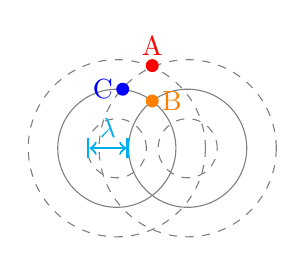
\begin{tikzpicture}[scale=1.5]
    \coordinate (A) at (-0.3,0);
    \coordinate (B) at (0.3,0);

    \draw[gray, dashed] (A) circle (0.25);
    \draw[gray] (A) circle (0.5);
    \draw[gray, dashed] (A) circle (0.75);

    \draw[gray, dashed] (B) circle (0.25);
    \draw[gray] (B) circle (0.5);
    \draw[gray, dashed] (B) circle (0.75);

    \filldraw[red] (0, 0.7) circle (0.05)
      node[above]{A};
    \filldraw[orange] (0, 0.4) circle (0.05)
      node[right]{B};
    \filldraw[blue] (-0.25, 0.5) circle (0.05)
      node[left]{C};

    \draw[|<->|, thick, cyan] (-0.2, 0) -- (-0.55, 0)
      node[pos=0.5, above]{$\lambda$};
  \end{tikzpicture}
\end{center}

In questa immagine sono stati segnati 3 punti. Nel punto \textcolor{red}{A} e nel punto 
\textcolor{orange}{B} si ha un'interferenza \textbf{costruttiva} in quando due ampiezze uguali
si incontrano.\\
Nel punto \textcolor{blue}{C} si ha un'interferenza \textbf{distruttiva} in quando due ampiezze diverse
si incontrano.

\subsubsection{Principio di Sovrapposizione}
\begin{center}
  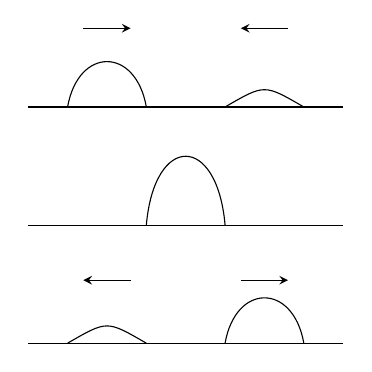
\begin{tikzpicture}
    \draw (0,0) -- ++(4,0);
    \draw (0.5,0) to[out=80, in = 100, looseness=2] (1.5,0);
    \draw (2.5,0) to[out=30, in = 150, looseness=1.5] (3.5,0);

    \draw[-stealth] (0.7,1) -- ++(0.6,0);
    \draw[-stealth] (3.3,1) -- ++(-0.6,0);

    \draw (0,-1.5) -- ++(4,0);
    \draw (1.5,-1.5) to[out=85, in = 95, looseness=3] (2.5,-1.5);

    \draw (0,-3) -- ++(4,0);
    \draw (2.5,-3) to[out=80, in = 100, looseness=2] (3.5,-3);
    \draw (0.5,-3) to[out=30, in = 150, looseness=1.5] (1.5,-3);

    \draw[-stealth] (1.3,-2.2) -- ++(-0.6,0);
    \draw[-stealth] (2.7,-2.2	) -- ++(+0.6,0);
  \end{tikzpicture}
\end{center}
\begin{equation*}
  y_{Tot} = y_1 + y_2
\end{equation*}

\subsubsection{Interferenza Costruttiva}
\begin{equation*}
  \left\lvert \overline{PS}_1-\overline{PS}_2 \right\rvert = k\mathcolor{cyan}{\lambda}
\end{equation*}
$\overline{PS}$: distanza tra l'origine dell'onda e il punto $P$\\
$k$: $k\in\mathbb{Z}$ indica il numero dell'interferenza che interessa, ovvero il numero dell'onda

\subsubsection{Interferenza Distruttiva}
\begin{equation*}
  \left\lvert \overline{PS}_1-\overline{PS}_2 \right\rvert = 
  \left( k+\frac{1}{2} \right)\mathcolor{cyan}{\lambda}
\end{equation*}
$\overline{PS}$: distanza tra l'origine dell'onda e il punto $P$\\
$k$: $k\in\mathbb{Z}$ indica il numero dell'interferenza che interessa, ovvero il numero dell'onda\\
[\baselineskip]

Nei punti di interferenza distruttiva, sommandosi ampiezza massima e minima vi sarà assenza di 
turbolenza.

\subsection{Esperienza di Young}\label{subsec:onde:young}
Young studiava la luce. Il suo esperimento dimostra la natura ondulatoria della luce. Di seguito
viene riportato un diagramma che rappresenta semplicemente la sua struttura.

\begin{center}
  \begin{tikzpicture}[xscale=0.8]
    \coordinate (MidL) at (-3.2, 0);
    \coordinate (MidR) at (3, 0);

    \coordinate (BlockTop) at (-2.8, 0.5);
    \coordinate (BlockBot) at (-2.8, -0.5);
    \coordinate (BlockMid) at (-2.8, 0);

    \coordinate (P) at (3, 1.5);

    \coordinate (MidBar) at (4.3, 0);

    \draw[dashed] (MidL) -- (MidR);
    \draw ($(P) + (0, 0.5)$) -- ++(0, -3.5);

    % Two holes
    \filldraw[lightgray, draw=black] 
      ($(BlockTop) + (0,0.5)$) -- (BlockTop) -- ++(-0.4, 0) -- ++(0, 0.5);
    \filldraw[lightgray, draw=black] 
      ($(BlockBot) + (0,-0.5)$) -- (BlockBot) -- ++(-0.4, 0) -- ++(0, -0.5);
    \filldraw[lightgray, draw=black] 
      ($(BlockMid) + (0,0.25)$) -- ($(BlockMid) + (0,-0.25)$) -- 
      ++(-0.4, 0) -- ++(0, 0.5) -- cycle;		

    % Lines to P
    \filldraw[black] (P) circle (0.05)
      node[right]{P};
    \draw[very thin] (BlockTop) -- (P);
    \draw (BlockMid) -- (P);
    \draw[very thin] (BlockBot) -- (P);

    % Delta x
    \draw[densely dotted] (BlockTop) -- ++(0.5, -0.84);
    \draw[|<->|] ($(BlockBot) + (0.2, -0.25)$) -- ($(BlockTop) + (0.6, -1.1)$)
      node[pos=0.5, below right]{$\Delta x =
      \mathcolor{red}{d}\sin\mathcolor{orange}{\theta_n}$};

    % Captions
    \filldraw[orange, fill=orange!50] (BlockMid) -- ++(1,0) arc(0:15:1) -- cycle;
    \draw[orange] (BlockMid) +(7:1.5) node{$\theta_n$};
    \draw[|<->|, blue] (-2.8, -1.5) -- ++(5.8, 0)
      node[pos=0.5, above]{$l$};
    \draw[|<->|] ($(P) + (0.5, 0)$) -- ++(0, -1.5)
      node[pos=0.5, right]{$y_n$};
    \draw[|<->|, red] ($(BlockTop) + (-0.9, 0)$) -- ++(0, -1)
      node[pos=0.5, right]{$d$};

    % Bar on right
    \coordinate (M) at ($(MidBar) + (0, 1.5)$);
    \foreach \y/\c in {0, 0.4, 0.8, ..., 3}{
      \filldraw[Violet] 
      ($(M) + (0,-\y)$) -- ++(0.5, 0) -- ++(0, -0.2) -- ++(-0.5, 0) -- cycle;
    }
    \foreach \y/\c in {0.2, 0.6, 1, ..., 2.6}{
      \filldraw[Goldenrod!50] 
      ($(M) + (0,-\y)$) -- ++(0.5, 0) -- ++(0, -0.2) -- ++(-0.5, 0) -- cycle;
    }
    \draw ($(MidBar) + (0,1.5)$) -- ++(0.5, 0) -- ++(0, -3) -- ++(-0.5, 0) -- cycle;

    \draw[|<->|, teal] ($(M) + (0.9, -0.3)$) -- ++(0, -0.4)
    node[pos=0.5, right]{$\frac{\mathcolor{blue}{l}\lambda}{\mathcolor{red}{d}}$};

    \node[Violet](C) at (1.5, -2) {Distruttiva};
    \node[Goldenrod] (C) at (1.5, -2.5) {Costruttiva};
  \end{tikzpicture}
\end{center}

La barra a destra fa vedere l'alternarsi di zone chiare e scure. Ciascuna di quelle zone è definita
\emph{frangia}.\\
Per gli esercizi si vada a pagina~\pageref{ex:young}.\\ [\baselineskip]
Secondo il principio di Huygens, ogni punto di un'onda è a sua volta sorgente di una. Ecco perché
dai fori, si sprigiona un'onda perfettamente circolare.

\subsubsection{Altezza dell'$n$-esima frangia}
La seguente formula trova l'altezza di una qualsiasi frangia.
\begin{equation*}
  y_n = \mathcolor{blue}{l}\tan\mathcolor{orange}{\theta_n}
\end{equation*}

Le prossime due invece trovano l'$n$-esima frangia costruttiva ($_C$) o distruttiva ($_D$).
\begin{equation*}
  y_{n_C} = \frac{\mathcolor{blue}{l}\cdot n\cdot\mathcolor{teal}{\lambda}}{\mathcolor{red}{d}}
\end{equation*}
\begin{equation*}
  y_{n_D} =
  \left(n+\frac{1}{2}\right)\frac{\mathcolor{blue}{l}\mathcolor{teal}{\lambda}}{\mathcolor{red}{d}}
\end{equation*}

\subsubsection{Angolo dell'$n$-esima frangia}
Se la frangia è costruttiva
\begin{equation*}
  \sin\mathcolor{orange}{\theta_n} = n\frac{\mathcolor{teal}{\lambda}}{\mathcolor{red}{d}}
\end{equation*}
Se è distruttiva
\begin{equation*}
  \sin\mathcolor{orange}{\theta_n} =
  \left(n+\frac{1}{2}\right)\frac{\mathcolor{teal}{\lambda}}{\mathcolor{red}{d}}
\end{equation*}

\subsubsection{Differenza di percorso tra i due fori}
\begin{equation*}
  \Delta x = \mathcolor{red}{d}\sin\mathcolor{orange}{\theta_n}
\end{equation*}
Se l'angolo è riferito ad una frangia costruttiva è 
\begin{equation*}
  \Delta x = n\mathcolor{teal}{\lambda}
\end{equation*}
Se l'angolo è riferito ad una frangia distruttiva è 
\begin{equation*}
  \Delta x = \left(n+\frac{1}{2}\right)\mathcolor{teal}{\lambda}
\end{equation*}

\subsection{Diffrazione}
\begin{center}
  \begin{tikzpicture}
    \coordinate (A) at (0,0);
    \coordinate (B) at (3,0);
    \coordinate (C) at (3,1);
    \coordinate (MidBar) at (3.5,0);
    \coordinate (P) at (3.5,0.6);

    \draw (0,1.5) -- ++(0,-1.4);
    \draw (0,-0.1) -- ++(0,-1);
    
    \draw[dashed] (A) -- (B);
    % Bar on right
    \coordinate (M) at ($(MidBar) + (0, 1.5)$);
    \foreach \y\c in {0, 0.4, 0.8, ..., 3}{
      \filldraw[Violet] 
      ($(M) + (0,-\y)$) -- ++(0.5, 0) -- ++(0, -0.2) -- ++(-0.5, 0) -- cycle;
    }
    \foreach \y/\c in {0.2, 0.6, 1, ..., 2.6}{
      \filldraw[Goldenrod!50] 
      ($(M) + (0,-\y)$) -- ++(0.5, 0) -- ++(0, -0.2) -- ++(-0.5, 0) -- cycle;
    }
    \draw ($(MidBar) + (0,1.5)$) -- ++(0.5, 0) -- ++(0, -3) -- ++(-0.5, 0) -- cycle;

    \draw (A) -- (P);
    \markangle{A}{B}{P}{1}{1.5}{$\theta_n$}
  \end{tikzpicture}
\end{center}

Se al posto di due fori ce ne fosse solo uno la prima frangia scura si troverebbe a $\theta$ gradi
dalla retta perpendicolare alle pareti
\begin{equation*}
  \theta = \arcsin\frac{n\lambda}{d}
\end{equation*}
$\lambda$: lunghezza d'onda\\
$d$: larghezza fenditura

\subsubsection{Reticolo di diffrazione}
Se invece ci fossero molti fori distanziati in maniera regolare, gli angoli per cui si riscontrano
frange chiare sono
\begin{equation*}
  \theta = \arcsin \frac{n\lambda}{d}
\end{equation*}
$n$: numero intero appartenente a $\mathbb{N}$\\
$\lambda$: lunghezza d'onda\\
$d$: distanza tra i fori

\subsection{Interferenza su lamine sottili}
La luce che incide su lamine sottili è in parte rifratta e in parte riflessa
\begin{center}
  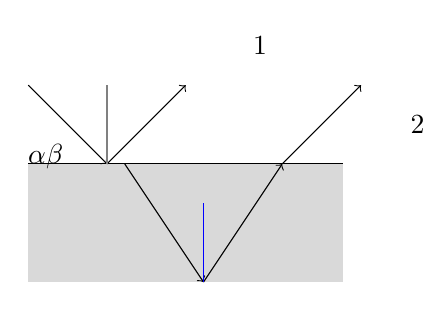
\begin{tikzpicture}
    \coordinate (O1) at (1,0);
    \coordinate (OO1) at (1,1);
    \coordinate (A1) at (0,1);
    \coordinate (B1) at (2,1);
    \coordinate (O2) at (2,-1.5);
    \coordinate (OO2) at (2,-0.5);
    \coordinate (A2) at (1,0);
    \coordinate (B2) at (3,0);
    \coordinate (C2) at (4,1);

    \draw (0,0) -- ++(4,0);
    \fill[gray, fill opacity = 0.3] (0,0) -- ++(4,0) -- ++(0,-1.5) -- ++(-4,0) -- cycle;
    
    \draw[->] (A1) -- (O1);
    \draw[->] (O1) -- (B1);
    \draw[thin,gray] (O1) -- (OO1);
    \markangle{O1}{A1}{OO1}{0.5}{1.4}{$\alpha$}

    \draw[->] (A2) -- (O2);
    \draw[->] (O2) -- (B2);
    \draw[->] (B2) -- (C2);
    \draw[thin,blue] (O2) -- (OO2);
    \markangle{O2}{A2}{OO2}{0.5}{1.4}{$\beta$}
    
    \node at (2.5,1.5) {1};
    \node at (4.5,0.5) {2};
  \end{tikzpicture}
\end{center}
I raggi 1 e 2 interagendo daranno luogo ad interferenza costruttiva se
\begin{equation*}
  D = \frac{\lambda}{2n} \left( m+\frac{1}{2} \right)
\end{equation*}
$D$: spessore\\
$\lambda$: lunghezza d'onda nel vuoto
$n$: indice di rifrazione
$m$: numero intero appartenente a $\mathbb{N}$

\subsection{Lenti e Specchi}\label{subsec:onde:lenti}
L'obiettivo fondamentale dell'ottica è mettere a fuoco degli oggetti. Generalmente si riscontrano
due problemi di vista: \emph{miopia} (difficoltà a mettere a fuoco lunghe distanze) e 
\emph{ipermetropia} (o presbiopia che è la difficoltà ad identificare oggetti vicini).\\
Per gli esercizi si vada a pagina~\pageref{ex:lenti}.\\ [\baselineskip]
Il disegno sotto aiuterà a capire i fondamenti dell'ottica
\begin{center}
  \begin{tikzpicture}
    \coordinate (p) at (-3, 0);
    \coordinate (hO) at (-3, 0.75);
    \coordinate (f) at (1.2, 0);
    \coordinate (L) at (0, 0);
    \coordinate (q) at (2, 0);
    \coordinate (hI) at (2, -0.5);

    % Construction
    \draw[very thin] (p) -- (q);
    \draw[red, thick] (p) -- (hO)
      node[pos=0.5, left]{$h_O$}
      node[pos=0, below]{$p$};
    \draw[blue, thick] (q) -- (hI)
      node[pos=0.5, right]{$h_I$}
      node[pos=0, above]{$q$};
    \draw[<->] ($(L) + (0, 1)$) -- ($(L) + (0, -1)$);

    % Connection lines
    \draw[dashed] (hO) -- (hI);
    \draw[densely dotted] (hO) -- ($(L) + (0, 0.75)$) -- (hI);

    % Sign for F
    \draw[orange, thick] ($(f) + (0, -0.2)$) -- ++(0, 0.4)
      node[pos=1, above]{$f$};
  \end{tikzpicture}
\end{center}

Per comprendere chiaramente il funzionamento di una lente è utile disegnare:
\begin{itemize}
  \item Una linea perpendicolare alla lente che viene deviata in modo da passare per il fuoco;
  \item Una linea passante per il centro della lente che continuerà il suo percorso senza 
    deviazioni;
\end{itemize}
Se queste due linee non si incontrano o l'immagine è virtuale o non c'è immagine.

\subsubsection{Equazione generale}
\begin{equation*}
  \frac{1}{\mathcolor{orange}{f}} = \frac{1}{\mathcolor{red}{p}} + \frac{1}{\mathcolor{blue}{q}}
\end{equation*}

\begin{center}
  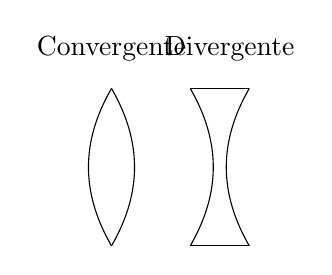
\begin{tikzpicture}
    \coordinate (A) at (0,1);
    \coordinate (B) at (0,-1);
    \coordinate (C) at (1,1);
    \coordinate (D) at (1.75,1);
    \coordinate (E) at (1,-1);
    \coordinate (F) at (1.75,-1);

    \path (A) edge[bend right] (B) (B) edge[bend right] (A);
    \path 
      (C) edge (D)
      (D) edge[bend right] (F)
      (F) edge (E)
      (E) edge[bend right] (C);

    \node at (0,1.5){Convergente};
    \node at (1.5,1.5){Divergente};
  \end{tikzpicture}
\end{center}
Per lenti sottili, si considera la convenzione che la distanza focale $f > 0$ per lenti convergenti
e $f<0$ per lenti divergenti. La distanza dell'oggetto $p$ è sempre positiva e la distanza dell'
immagine è positiva quando $q$ è dall'altro lato della lente.\\
Un'immagine virtuale ha $q < 0$. L'ingrandimento è positivo per un'immagine dritta e negativo per una
rovesciata.

\subsubsection{Ingrandimento}
\begin{equation*}
  G = \frac{\mathcolor{red}{h_I}}{\mathcolor{blue}{h_O}} =
  -\frac{\mathcolor{blue}{q}}{\mathcolor{red}{p}}
\end{equation*}

\subsubsection{Diottria}
Nell'ottica, per trovare la distanza focale della lente da usare negli occhiali, si usi
\begin{align*}
  \text{Miopia:}\,\frac{1}{f}&=\frac{1}{d}-\frac{1}{d_{max}}\\
  \text{Ipermetropia:}\,\frac{1}{f}&=\frac{1}{d}-\frac{1}{d_{min}} 
\end{align*}
dove $d$ è la distanza da ottenere.
$d_{max}$: massima distanza a cui si vede chiaramente\\
$d_{min}$: minima distanza a cui si vede chiaramente

\subsubsection{Lenti attaccate}
Se due lenti di distanza focale $f_1$ e $f_2$ sono attaccate, possono essere sostituite da una sola
di distanza focale $f$.
\begin{equation*}
  \frac{1}{f} = \frac{1}{f_1}+\frac{1}{f_2}
\end{equation*}

\subsection{Specchi}
Per gli specchi valgono le stesse leggi delle lenti.\\
Si definisce \emph{concavo} se $f>0$ e \emph{convesso} altrimenti. 
\begin{center}
  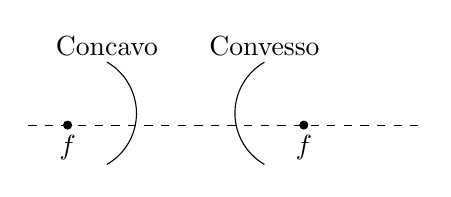
\begin{tikzpicture}
    \draw[dashed] (0,0) -- (5,0);
    \draw (1,0.8) arc (60:-60:0.75);
    \draw (3,-0.5) arc (60:-60:-0.75);
    \filldraw (0.5,0) circle (0.05)
      node[below]{$f$};
    \filldraw (3.5,0) circle (0.05)
      node[below]{$f$};
    \node at (1,1){Concavo};
    \node at (3,1){Convesso};
  \end{tikzpicture}
\end{center}
\begin{equation*}
  f = \frac{R}{2}
\end{equation*}


\subsection{Onde Stazionarie}
Si possono riscontrare onde stazionarie quando due onde siano sincrone ma con versi opposti. Il 
risultato è il seguente

\begin{center}
  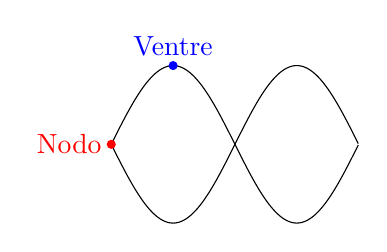
\begin{tikzpicture}
    \draw[samples=500, domain=-0:pi] plot (\x, {-sin(2*\x r)});
    \draw[samples=500, domain=-0:pi] plot (\x, {sin(2*\x r)});

    \filldraw[red] (0,0) circle(0.05)
      node[left]{Nodo};
    \filldraw[blue] (pi/4, 1) circle(0.05)
      node[above]{Ventre};
  \end{tikzpicture}
\end{center}

Per le onde stazionarie, vengono definiti \emph{nodi} i punti in cui l'ampiezza è  $0$,
\emph{ventri} quelli in cui l'ampiezza è massima. Si definisce $n$ il numero di ventri che 
esistono nell'onda.\\
Per trovare la posizione di un nodo o di un ventre si usi
\begin{equation*}
  \mathcolor{red}{\text{Nodo: }} x = \frac{\lambda}{4}+(k+1)\frac{\lambda}{2}
\end{equation*}
\begin{equation*}
  \mathcolor{blue}{\text{Ventre: }} x = (k+1)\frac{\lambda}{2}
\end{equation*}
dove $k$ identifica il numero del ventre o nodo desiderato.

\begin{center}
  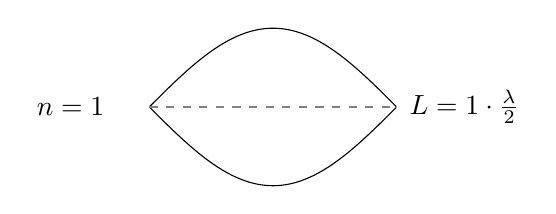
\begin{tikzpicture}
    \node at (-1,0){$n=1$};
    \node at (4,0){$L=1\cdot\frac{\lambda}{2}$};
    \draw[samples=500, domain=-0:pi] plot (\x, {-sin(\x r)});
    \draw[samples=500, domain=-0:pi] plot (\x, {sin(\x r)});
    \draw[gray, dashed] (0,0) -- ++(3.14,0);
  \end{tikzpicture}
\end{center}
\begin{center}
  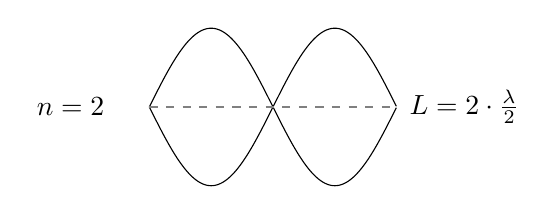
\begin{tikzpicture}
    \node at (-1,0){$n=2$};
    \node at (4,0){$L=2\cdot\frac{\lambda}{2}$};
    \draw[samples=500, domain=-0:pi] plot (\x, {-sin(2*\x r)});
    \draw[samples=500, domain=-0:pi] plot (\x, {sin(2*\x r)});
    \draw[gray, dashed] (0,0) -- ++(3.14,0);
  \end{tikzpicture}
\end{center}
\begin{center}
  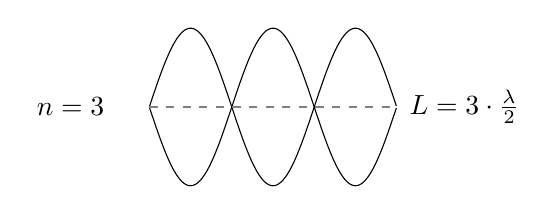
\begin{tikzpicture}
    \node at (-1,0){$n=3$};
    \node at (4,0){$L=3\cdot\frac{\lambda}{2}$};
    \draw[samples=500, domain=-0:pi] plot (\x, {-sin(3*\x r)});
    \draw[samples=500, domain=-0:pi] plot (\x, {sin(3*\x r)});
    \draw[gray, dashed] (0,0) -- ++(3.14,0);
  \end{tikzpicture}
\end{center}

\subsubsection{Equazione dell'onda stazionaria}
\begin{equation*}
  y = A\cos\left(\frac{2\pi x}{\lambda}\right)\sin\left(\frac{2\pi t}{T}\right)
\end{equation*}

\subsubsection{Lunghezza dell'onda}
La lunghezza dell'onda è determinata da $n$ e dalla lunghezza d'onda.
\begin{equation*}
  L = n\frac{\lambda_n}{2}
\end{equation*}
Dove $\lambda_n$ è definita come
\begin{equation*}
  \lambda_n = \frac{2L}{n}
\end{equation*}

\subsubsection{Frequenza del ventre}
\begin{equation*}
  f_n = \frac{n}{2L}v
\end{equation*}
$v$: velocità (che può essere espressa come $\sqrt{\frac{T}{\mu}}$)

\subsection{Suono}\label{subsec:onde:suono}
Il suono è un'onda meccanica, quindi rientra in questa sezione. Il suono si propaga in forma
sferica da un punto.\\[\baselineskip]
Per gli esercizi, si vada a pagina~\pageref{ex:suono}.

\subsubsection{Intensità}
L'intensità indica quanto forte è un suono. \\
Dato che il suono si propaga in forma sferica, 
$S = 4\pi r^2$ dove $r$ indica la distanza dell'uditore dalla sorgente.
\begin{equation*}
  I = \frac{E}{St} = \frac{P}{S}
\end{equation*}
$E$: energia\\
$P$: potenza, solitamente espressa in $W$\\[\baselineskip]
Se ne deriva che
\begin{equation*}
  I_1r_1^2 = I_2r_2^2
\end{equation*}
\begin{center}
  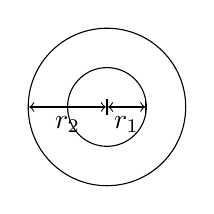
\begin{tikzpicture}[scale=0.5]
    \draw (0,0) circle (1);
    \draw (0,0) circle (2);
    \draw[|<->|] (0,0) -- ++(1,0)
      node[pos=0.5,below]{$r_1$};
    \draw[|<->|] (0,0) -- ++(-2,0)
      node[pos=0.5,below]{$r_2$};
  \end{tikzpicture}
\end{center}


\subsubsection{Livello sonoro}
Il livello sonoro indica quanto forte un suono appare all'udito umano. La sua unità di misura è il
\emph{decibel} ($dB$).

\begin{equation*}
  L = 10\log_{10}\frac{I}{I_0}
\end{equation*}
\hyperref[tab:I0]{$I_0$}: $10^{-12}\,\text{W/m}^2$

\subsubsection{Eco}
Il suono, essendo un onda, si riflette se incontra un ostacolo. Il tempo necessario tra due picchi
perché si senta l'eco è
\begin{equation*}
  t = \frac{2d}{v}
\end{equation*}
\begin{center}
  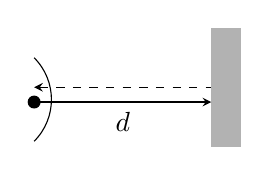
\begin{tikzpicture}[scale=0.75]
    \filldraw[gray!60] (3,0) -- ++(0.5,0) -- ++(0,2) -- ++(-0.5,0) -- cycle;
    \draw (0,1.5) arc (45:-45:1);
    \filldraw (0,0.75) circle (0.1);
    \draw[-stealth] (0,0.75) -- ++(3,0)
      node[pos=0.5,below]{$d$};
    \draw[stealth-,dashed] (0,1) -- ++(3,0);
  \end{tikzpicture}
\end{center}
$d$: distanza dalla superficie\\
\hyperref[tab:vs]{$v$}: $343$ m/s

\subsubsection{Effetto Doppler}
L'effetto Doppler è un effetto che tutti quanti conoscono (un'ambulanza che emette un 
suono diverso in base alla sua velocità relativa rispetto all'uditore) e che mette in relazione la 
frequenza del suono e la velocità dei due corpi (uditore e sorgente).\\

La cosa più complicata dell'effetto Doppler sono i segni. Questa è la formula più generale
\begin{equation*}
  f_O = f_S\frac{v\pm v_U}{v\mp v_S}
\end{equation*}
\hyperref[tab:vs]{$v$}: $343\,\text{m/s}$\\
$U$: uditore\\
$S$: sorgente\\

Come si nota, al numeratore e al denominatore si invertono i segni. Questa tabella aiuterà a far 
capire come scegliere.

\begin{center}
  \begin{tabular}{| c | c | c |}
    \hline
    \multicolumn{1}{|c}{\multirow{2}{*}{Uditore}} & 
    \multicolumn{1}{|c|}{Avvicina} & $+$\\ \cline{2-3}
    \multicolumn{1}{|c}{} &
    \multicolumn{1}{|c|}{Allontana} & $-$\\ 
    \hline\hline
    \multicolumn{1}{|c}{\multirow{2}{*}{Sorgente}} & 
    \multicolumn{1}{|c|}{Avvicina} & $-$\\ \cline{2-3}
    \multicolumn{1}{|c}{} &
    \multicolumn{1}{|c|}{Allontana} & $+$\\
    \hline 
  \end{tabular}
\end{center}

La formula vale anche quando entrambi i corpi sono in movimento. Se l'uditore o la sorgente sono fermi
rispettivamente $v_U$ e $v_S$ sono pari a $0$.

\subsubsection{Battimenti}
I battimenti sono un fenomeno che si verifica quando due sorgenti vibrano a frequenze molto simili,
quindi $f_1 \approx f_2$. Se questa condizione non è presente, non è un battimento.\\
Un tipico esempio è un diapason che comincia a vibrare quando si canta alla giusta tonalità.

\begin{equation*}
  f_B = \left\vert f_1 - f_2 \right\vert
\end{equation*}
